%%
% The SUEPThesis Template for Bachelor Graduation Thesis
%
% 上海电力大学毕业设计(论文)中英文摘要 —— 使用 XeLaTeX 编译
%
% Copyright 2020-2023 SUEPaper
%
% This work may be distributed and/or modified under the
% conditions of the LaTeX Project Public License, either version 1.3
% of this license or (at your option) any later version.
% The latest version of this license is in
%   http://www.latex-project.org/lppl.txt
% and version 1.3 or later is part of all distributions of LaTeX
% version 2005/12/01 or later.
%
% This work has the LPPL maintenance status `maintained'.
%
% The Current Maintainer of this work is Haiwen Zhang.
%%

\chapter{不同情形WPCR生产和存储模型的综合分析}

\section{不同情形的WPCR生产和存储总成本比较}

通过前面四个模型优化结果可知,连续多周生产统筹规划模型相较于不允许缺货的WPCR生产和存储模型增加组装迟滞,
由图表可以看出其费用大大升高,对研究组装分配计划具有重要现实意义。
考虑检修的生产和存储模型和WPCR不确定生产和存储模型在连续多周生产统筹规划模型的基础上展开,
分别得出增设检修日期和需求未知条件下的最小费用,经对比分析,可对复杂生产中组装计划的调度具有指导意义。

\begin{figure}[h]
    \centering
    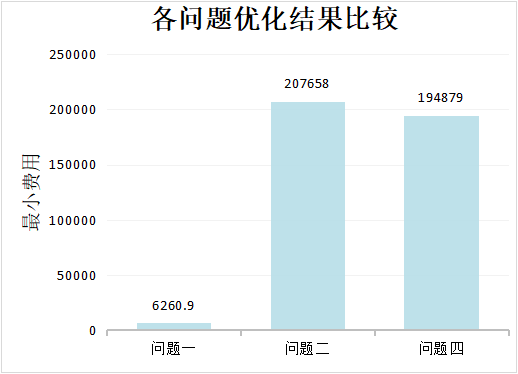
\includegraphics[width=0.7\linewidth]{ch6-1.png}
    \caption{各问题优化结果比较}
    \label{f.ch6-1}
\end{figure}

\section{不同情形的WPCR生产和存储求解的灵敏度分析}

经过灵敏度分析验证,通过遗传算法的迭代次数,以及种群数、变异率、交叉率以求得最短运行时间下的最优结果,
得出模型运算灵敏度分析,模型在大于150次迭代运算的情况下运行结果基本一致,在策略迭代中采取大种群,
在费用估计中可用最优变异交叉率来节省运算时间来求得全局最优解和动态稳定解。

\begin{figure}[H]
    \centering
    \begin{subfigure}[t]{0.5\linewidth}
        \captionsetup{justification=centering}
        \begin{minipage}[b]{1\linewidth}
            \centering
            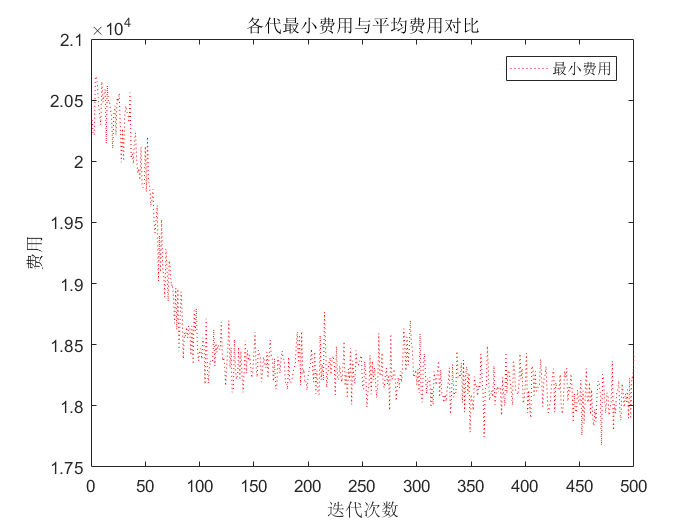
\includegraphics[width=0.8\linewidth]{ch6-2-1.png}
            \caption{}
        \end{minipage}
    \end{subfigure}
    \hspace{-5em}
    \begin{subfigure}[t]{0.5\linewidth}
        \captionsetup{justification=centering}
        \begin{minipage}[b]{1\linewidth}
            \centering
            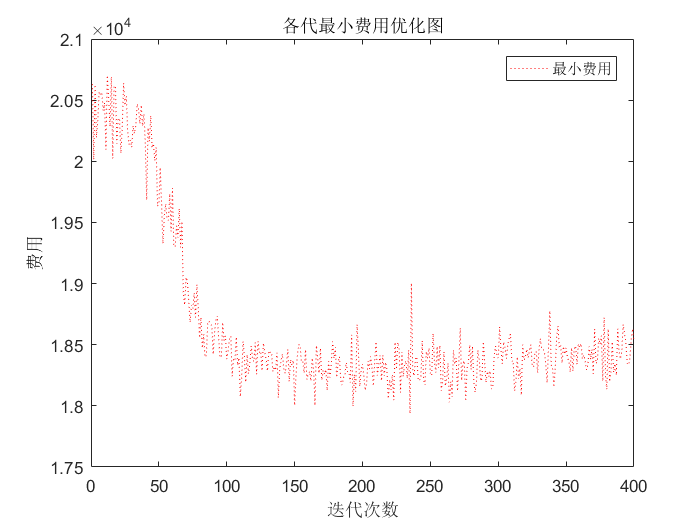
\includegraphics[width=0.8\linewidth]{ch6-2-2.png}
            \caption{}
        \end{minipage}
    \end{subfigure}\\
    \begin{subfigure}[t]{0.5\linewidth}
        \captionsetup{justification=centering}
        \begin{minipage}[b]{1\linewidth}
            \centering
            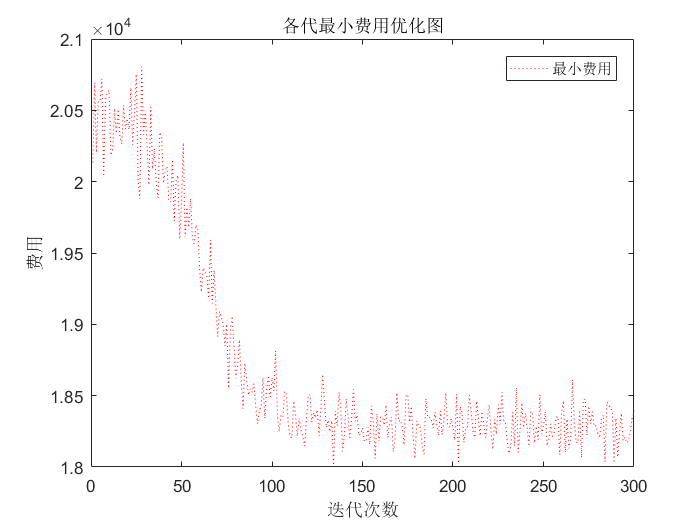
\includegraphics[width=0.8\linewidth]{ch6-2-3.png}
            \caption{}
        \end{minipage}
    \end{subfigure}
    \hspace{-5em}
    \begin{subfigure}[t]{0.5\linewidth}
        \captionsetup{justification=centering}
        \begin{minipage}[b]{1\linewidth}
            \centering
            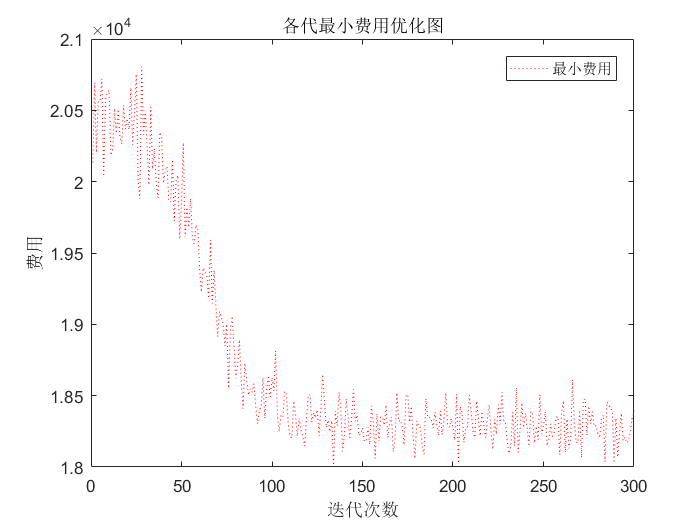
\includegraphics[width=0.8\linewidth]{ch6-2-3.png}
            \caption{}
        \end{minipage}
    \end{subfigure}
    \caption{不同迭代次数对比}
    \label{f.ch6-2}
\end{figure}